\PassOptionsToPackage{unicode=true}{hyperref} % options for packages loaded elsewhere
\PassOptionsToPackage{hyphens}{url}
%
\documentclass[]{article}
\usepackage{lmodern}
\usepackage{amssymb,amsmath}
\usepackage{ifxetex,ifluatex}
\usepackage{fixltx2e} % provides \textsubscript
\ifnum 0\ifxetex 1\fi\ifluatex 1\fi=0 % if pdftex
  \usepackage[T1]{fontenc}
  \usepackage[utf8]{inputenc}
  \usepackage{textcomp} % provides euro and other symbols
\else % if luatex or xelatex
  \usepackage{unicode-math}
  \defaultfontfeatures{Ligatures=TeX,Scale=MatchLowercase}
\fi
% use upquote if available, for straight quotes in verbatim environments
\IfFileExists{upquote.sty}{\usepackage{upquote}}{}
% use microtype if available
\IfFileExists{microtype.sty}{%
\usepackage[]{microtype}
\UseMicrotypeSet[protrusion]{basicmath} % disable protrusion for tt fonts
}{}
\IfFileExists{parskip.sty}{%
\usepackage{parskip}
}{% else
\setlength{\parindent}{0pt}
\setlength{\parskip}{6pt plus 2pt minus 1pt}
}
\usepackage{hyperref}
\hypersetup{
            pdftitle={SimpleLinearRegressionCustomAlgorithm},
            pdfauthor={bneella},
            pdfborder={0 0 0},
            breaklinks=true}
\urlstyle{same}  % don't use monospace font for urls
\usepackage[margin=1in]{geometry}
\usepackage{color}
\usepackage{fancyvrb}
\newcommand{\VerbBar}{|}
\newcommand{\VERB}{\Verb[commandchars=\\\{\}]}
\DefineVerbatimEnvironment{Highlighting}{Verbatim}{commandchars=\\\{\}}
% Add ',fontsize=\small' for more characters per line
\usepackage{framed}
\definecolor{shadecolor}{RGB}{248,248,248}
\newenvironment{Shaded}{\begin{snugshade}}{\end{snugshade}}
\newcommand{\AlertTok}[1]{\textcolor[rgb]{0.94,0.16,0.16}{#1}}
\newcommand{\AnnotationTok}[1]{\textcolor[rgb]{0.56,0.35,0.01}{\textbf{\textit{#1}}}}
\newcommand{\AttributeTok}[1]{\textcolor[rgb]{0.77,0.63,0.00}{#1}}
\newcommand{\BaseNTok}[1]{\textcolor[rgb]{0.00,0.00,0.81}{#1}}
\newcommand{\BuiltInTok}[1]{#1}
\newcommand{\CharTok}[1]{\textcolor[rgb]{0.31,0.60,0.02}{#1}}
\newcommand{\CommentTok}[1]{\textcolor[rgb]{0.56,0.35,0.01}{\textit{#1}}}
\newcommand{\CommentVarTok}[1]{\textcolor[rgb]{0.56,0.35,0.01}{\textbf{\textit{#1}}}}
\newcommand{\ConstantTok}[1]{\textcolor[rgb]{0.00,0.00,0.00}{#1}}
\newcommand{\ControlFlowTok}[1]{\textcolor[rgb]{0.13,0.29,0.53}{\textbf{#1}}}
\newcommand{\DataTypeTok}[1]{\textcolor[rgb]{0.13,0.29,0.53}{#1}}
\newcommand{\DecValTok}[1]{\textcolor[rgb]{0.00,0.00,0.81}{#1}}
\newcommand{\DocumentationTok}[1]{\textcolor[rgb]{0.56,0.35,0.01}{\textbf{\textit{#1}}}}
\newcommand{\ErrorTok}[1]{\textcolor[rgb]{0.64,0.00,0.00}{\textbf{#1}}}
\newcommand{\ExtensionTok}[1]{#1}
\newcommand{\FloatTok}[1]{\textcolor[rgb]{0.00,0.00,0.81}{#1}}
\newcommand{\FunctionTok}[1]{\textcolor[rgb]{0.00,0.00,0.00}{#1}}
\newcommand{\ImportTok}[1]{#1}
\newcommand{\InformationTok}[1]{\textcolor[rgb]{0.56,0.35,0.01}{\textbf{\textit{#1}}}}
\newcommand{\KeywordTok}[1]{\textcolor[rgb]{0.13,0.29,0.53}{\textbf{#1}}}
\newcommand{\NormalTok}[1]{#1}
\newcommand{\OperatorTok}[1]{\textcolor[rgb]{0.81,0.36,0.00}{\textbf{#1}}}
\newcommand{\OtherTok}[1]{\textcolor[rgb]{0.56,0.35,0.01}{#1}}
\newcommand{\PreprocessorTok}[1]{\textcolor[rgb]{0.56,0.35,0.01}{\textit{#1}}}
\newcommand{\RegionMarkerTok}[1]{#1}
\newcommand{\SpecialCharTok}[1]{\textcolor[rgb]{0.00,0.00,0.00}{#1}}
\newcommand{\SpecialStringTok}[1]{\textcolor[rgb]{0.31,0.60,0.02}{#1}}
\newcommand{\StringTok}[1]{\textcolor[rgb]{0.31,0.60,0.02}{#1}}
\newcommand{\VariableTok}[1]{\textcolor[rgb]{0.00,0.00,0.00}{#1}}
\newcommand{\VerbatimStringTok}[1]{\textcolor[rgb]{0.31,0.60,0.02}{#1}}
\newcommand{\WarningTok}[1]{\textcolor[rgb]{0.56,0.35,0.01}{\textbf{\textit{#1}}}}
\usepackage{graphicx,grffile}
\makeatletter
\def\maxwidth{\ifdim\Gin@nat@width>\linewidth\linewidth\else\Gin@nat@width\fi}
\def\maxheight{\ifdim\Gin@nat@height>\textheight\textheight\else\Gin@nat@height\fi}
\makeatother
% Scale images if necessary, so that they will not overflow the page
% margins by default, and it is still possible to overwrite the defaults
% using explicit options in \includegraphics[width, height, ...]{}
\setkeys{Gin}{width=\maxwidth,height=\maxheight,keepaspectratio}
\setlength{\emergencystretch}{3em}  % prevent overfull lines
\providecommand{\tightlist}{%
  \setlength{\itemsep}{0pt}\setlength{\parskip}{0pt}}
\setcounter{secnumdepth}{0}
% Redefines (sub)paragraphs to behave more like sections
\ifx\paragraph\undefined\else
\let\oldparagraph\paragraph
\renewcommand{\paragraph}[1]{\oldparagraph{#1}\mbox{}}
\fi
\ifx\subparagraph\undefined\else
\let\oldsubparagraph\subparagraph
\renewcommand{\subparagraph}[1]{\oldsubparagraph{#1}\mbox{}}
\fi

% set default figure placement to htbp
\makeatletter
\def\fps@figure{htbp}
\makeatother


\title{SimpleLinearRegressionCustomAlgorithm}
\author{bneella}
\date{15/01/2020}

\begin{document}
\maketitle

\hypertarget{agenda}{%
\section{AGENDA:}\label{agenda}}

\hypertarget{understand-the-problem-statement}{%
\section{Understand the problem
statement}\label{understand-the-problem-statement}}

\hypertarget{understand-the-data}{%
\section{Understand the data}\label{understand-the-data}}

\hypertarget{eda---exploratory-data-analysis}{%
\section{EDA - Exploratory Data
Analysis}\label{eda---exploratory-data-analysis}}

\hypertarget{clean-and-process-the-data}{%
\section{Clean and process the data}\label{clean-and-process-the-data}}

\hypertarget{model-the-data}{%
\section{Model the data}\label{model-the-data}}

\hypertarget{evaluation-and-communiacation}{%
\section{Evaluation and
Communiacation}\label{evaluation-and-communiacation}}

\begin{Shaded}
\begin{Highlighting}[]
\NormalTok{knitr}\OperatorTok{::}\NormalTok{opts_chunk}\OperatorTok{$}\KeywordTok{set}\NormalTok{(}\DataTypeTok{echo =} \OtherTok{TRUE}\NormalTok{)}
\NormalTok{knitr}\OperatorTok{::}\KeywordTok{include_graphics}\NormalTok{(}\StringTok{'/Images/slope.PNG'}\NormalTok{)}
\end{Highlighting}
\end{Shaded}

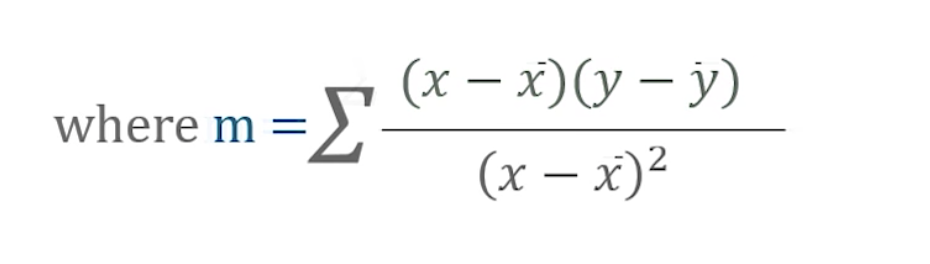
\includegraphics{/Images/slope.PNG}

\begin{Shaded}
\begin{Highlighting}[]
\NormalTok{knitr}\OperatorTok{::}\KeywordTok{include_graphics}\NormalTok{(}\StringTok{'/Images/r_squared.PNG'}\NormalTok{)}
\end{Highlighting}
\end{Shaded}

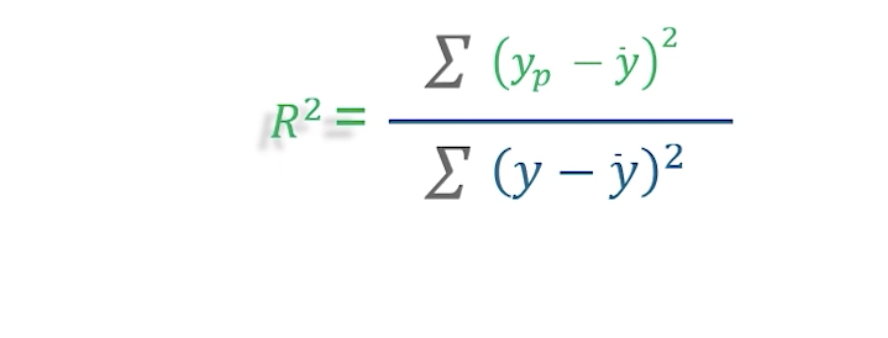
\includegraphics{/Images/r_squared.PNG}

\hypertarget{r-markdown}{%
\subsection{R Markdown}\label{r-markdown}}

This is an R Markdown document. Markdown is a simple formatting syntax
for authoring HTML, PDF, and MS Word documents. For more details on
using R Markdown see \url{http://rmarkdown.rstudio.com}.

When you click the \textbf{Knit} button a document will be generated
that includes both content as well as the output of any embedded R code
chunks within the document. You can embed an R code chunk like this:

\hypertarget{lets-first-clear-the-local-environment-before-starting}{%
\subsection{Let's first clear the local environment before
starting}\label{lets-first-clear-the-local-environment-before-starting}}

\begin{Shaded}
\begin{Highlighting}[]
\KeywordTok{rm}\NormalTok{(}\DataTypeTok{list =} \KeywordTok{ls}\NormalTok{(}\DataTypeTok{all=}\OtherTok{TRUE}\NormalTok{))}
\end{Highlighting}
\end{Shaded}

\hypertarget{import-data-file}{%
\subsection{Import data file}\label{import-data-file}}

\begin{Shaded}
\begin{Highlighting}[]
\NormalTok{data_set =}\StringTok{ }\KeywordTok{read.csv}\NormalTok{(}\StringTok{'Toyota_SimpleReg.csv'}\NormalTok{)}
\KeywordTok{head}\NormalTok{(data_set)}
\end{Highlighting}
\end{Shaded}

\begin{verbatim}
##   Id                                             Model Price Age_06_15
## 1  1     TOYOTA Corolla 2.0 D4D HATCHB TERRA 2/3-Doors 13500        57
## 2  2     TOYOTA Corolla 2.0 D4D HATCHB TERRA 2/3-Doors 13750        57
## 3  3 \xa0TOYOTA Corolla 2.0 D4D HATCHB TERRA 2/3-Doors 13950        58
## 4  4     TOYOTA Corolla 2.0 D4D HATCHB TERRA 2/3-Doors 14950        60
## 5  5       TOYOTA Corolla 2.0 D4D HATCHB SOL 2/3-Doors 13750        64
## 6  6       TOYOTA Corolla 2.0 D4D HATCHB SOL 2/3-Doors 12950        66
\end{verbatim}

\hypertarget{lets-rename-column-age_06_15-to-just-age-for-better-readability}{%
\subsection{Lets rename column `Age\_06\_15' to just `Age' for better
readability}\label{lets-rename-column-age_06_15-to-just-age-for-better-readability}}

\begin{Shaded}
\begin{Highlighting}[]
\KeywordTok{names}\NormalTok{(data_set)[}\DecValTok{4}\NormalTok{] =}\StringTok{ 'Age'}
\KeywordTok{head}\NormalTok{(data_set)}
\end{Highlighting}
\end{Shaded}

\begin{verbatim}
##   Id                                             Model Price Age
## 1  1     TOYOTA Corolla 2.0 D4D HATCHB TERRA 2/3-Doors 13500  57
## 2  2     TOYOTA Corolla 2.0 D4D HATCHB TERRA 2/3-Doors 13750  57
## 3  3 \xa0TOYOTA Corolla 2.0 D4D HATCHB TERRA 2/3-Doors 13950  58
## 4  4     TOYOTA Corolla 2.0 D4D HATCHB TERRA 2/3-Doors 14950  60
## 5  5       TOYOTA Corolla 2.0 D4D HATCHB SOL 2/3-Doors 13750  64
## 6  6       TOYOTA Corolla 2.0 D4D HATCHB SOL 2/3-Doors 12950  66
\end{verbatim}

\hypertarget{drop-columns-id-and-model}{%
\subsection{Drop columns `Id' and
`Model'}\label{drop-columns-id-and-model}}

\begin{Shaded}
\begin{Highlighting}[]
\NormalTok{columns_to_drop =}\StringTok{ }\KeywordTok{c}\NormalTok{(}\StringTok{'Id'}\NormalTok{, }\StringTok{'Model'}\NormalTok{)}
\NormalTok{data_set[columns_to_drop] =}\StringTok{ }\OtherTok{NULL}
\KeywordTok{head}\NormalTok{(data_set)}
\end{Highlighting}
\end{Shaded}

\begin{verbatim}
##   Price Age
## 1 13500  57
## 2 13750  57
## 3 13950  58
## 4 14950  60
## 5 13750  64
## 6 12950  66
\end{verbatim}

\hypertarget{lets-check-if-there-are-any-na-values}{%
\subsection{Lets check if there are any na
values}\label{lets-check-if-there-are-any-na-values}}

\begin{Shaded}
\begin{Highlighting}[]
\KeywordTok{sum}\NormalTok{(}\KeywordTok{is.na}\NormalTok{(data_set))}
\end{Highlighting}
\end{Shaded}

\begin{verbatim}
## [1] 0
\end{verbatim}

\hypertarget{scatter-plot-pricey-vs-agex}{%
\subsection{Scatter plot Price(y) vs
Age(x)}\label{scatter-plot-pricey-vs-agex}}

\begin{Shaded}
\begin{Highlighting}[]
\KeywordTok{plot}\NormalTok{(data_set}\OperatorTok{$}\NormalTok{Age, data_set}\OperatorTok{$}\NormalTok{Price, }\DataTypeTok{main =} \StringTok{'Price Vs Age'}\NormalTok{, }\DataTypeTok{xlab =} \StringTok{'Age'}\NormalTok{, }\DataTypeTok{ylab =} \StringTok{'Price'}\NormalTok{)}
\end{Highlighting}
\end{Shaded}

\includegraphics{SimpleLinearRegressionCustomAlgorithm_files/figure-latex/unnamed-chunk-6-1.pdf}

\hypertarget{let-us-see-the-covariance-of-the-price-and-age-to-understand-their-relationship}{%
\subsection{Let us see the covariance of the price and age to understand
their
relationship}\label{let-us-see-the-covariance-of-the-price-and-age-to-understand-their-relationship}}

\hypertarget{suggests-that-they-are-highly-inversely-proportional-to-eachother}{%
\subsection{-59136.11 suggests that they are highly inversely
proportional to
eachother}\label{suggests-that-they-are-highly-inversely-proportional-to-eachother}}

\begin{Shaded}
\begin{Highlighting}[]
\KeywordTok{cov}\NormalTok{(data_set}\OperatorTok{$}\NormalTok{Age, data_set}\OperatorTok{$}\NormalTok{Price)}
\end{Highlighting}
\end{Shaded}

\begin{verbatim}
## [1] -59136.11
\end{verbatim}

\hypertarget{let-us-see-the-correlation-of-the-price-and-age-to-understand-the-strength-of-their-relationship}{%
\subsection{Let us see the correlation of the price and age to
understand the strength of their
relationship}\label{let-us-see-the-correlation-of-the-price-and-age-to-understand-the-strength-of-their-relationship}}

\hypertarget{suggests-that-there-is-a-strong-negative-relationship}{%
\subsection{-0.8765905 suggests that there is a strong negative
relationship}\label{suggests-that-there-is-a-strong-negative-relationship}}

\begin{Shaded}
\begin{Highlighting}[]
\NormalTok{cor_data =}\StringTok{ }\KeywordTok{cor}\NormalTok{(data_set}\OperatorTok{$}\NormalTok{Age, data_set}\OperatorTok{$}\NormalTok{Price)}
\NormalTok{cor_data}
\end{Highlighting}
\end{Shaded}

\begin{verbatim}
## [1] -0.8765905
\end{verbatim}

\hypertarget{let-us-now-split-70-of-the-available-data-to-train-the-model-by-selecting-any-of-the-columns-we-have-availavle}{%
\subsection{Let us now split 70\% of the available data to train the
model by selecting any of the columns we have
availavle}\label{let-us-now-split-70-of-the-available-data-to-train-the-model-by-selecting-any-of-the-columns-we-have-availavle}}

\begin{Shaded}
\begin{Highlighting}[]
\KeywordTok{library}\NormalTok{(caret)}
\end{Highlighting}
\end{Shaded}

\begin{verbatim}
## Loading required package: lattice
\end{verbatim}

\begin{verbatim}
## Loading required package: ggplot2
\end{verbatim}

\begin{Shaded}
\begin{Highlighting}[]
\NormalTok{train_data_rows =}\StringTok{ }\KeywordTok{createDataPartition}\NormalTok{(data_set}\OperatorTok{$}\NormalTok{Price, }\DataTypeTok{p =} \FloatTok{0.7}\NormalTok{, }\DataTypeTok{list =} \OtherTok{FALSE}\NormalTok{)}
\NormalTok{train_data_set =}\StringTok{ }\NormalTok{data_set[train_data_rows, ]}
\NormalTok{test_data_set =}\StringTok{ }\NormalTok{data_set[}\OperatorTok{-}\NormalTok{train_data_rows, ]}
\KeywordTok{head}\NormalTok{(train_data_set)}
\end{Highlighting}
\end{Shaded}

\begin{verbatim}
##   Price Age
## 2 13750  57
## 3 13950  58
## 5 13750  64
## 6 12950  66
## 7 16900  61
## 9 21500  61
\end{verbatim}

\begin{Shaded}
\begin{Highlighting}[]
\KeywordTok{head}\NormalTok{(test_data_set)}
\end{Highlighting}
\end{Shaded}

\begin{verbatim}
##    Price Age
## 1  13500  57
## 4  14950  60
## 8  18600  64
## 10 12950  57
## 12 19950  56
## 18 17950  58
\end{verbatim}

\hypertarget{let-us-try-building-the-simple-linear-regression-algorithm}{%
\subsection{Let us try building the Simple Linear Regression
Algorithm}\label{let-us-try-building-the-simple-linear-regression-algorithm}}

\hypertarget{step-1-create-a-data-frame-with-x-and-y}{%
\subsection{step 1: create a data frame with x and
y}\label{step-1-create-a-data-frame-with-x-and-y}}

\begin{Shaded}
\begin{Highlighting}[]
\NormalTok{my_df =}\StringTok{ }\KeywordTok{data.frame}\NormalTok{(}\DataTypeTok{Age =}\NormalTok{ train_data_set}\OperatorTok{$}\NormalTok{Age, }\DataTypeTok{Price =}\NormalTok{ train_data_set}\OperatorTok{$}\NormalTok{Price)}
\NormalTok{my_df}
\end{Highlighting}
\end{Shaded}

\begin{verbatim}
##      Age Price
## 1     57 13750
## 2     58 13950
## 3     64 13750
## 4     66 12950
## 5     61 16900
## 6     61 21500
## 7     59 20950
## 8     59 19600
## 9     65 21500
## 10    66 22500
## 11    62 22000
## 12    64 22750
## 13    58 16750
## 14    64 16950
## 15    64 15950
## 16    62 15950
## 17    62 16950
## 18    63 16250
## 19    59 15950
## 20    61 17495
## 21    63 15750
## 22    62 16950
## 23    64 17950
## 24    63 12950
## 25    56 15750
## 26    61 15950
## 27    60 14950
## 28    56 15500
## 29    60 15750
## 30    66 15750
## 31    61 14750
## 32    56 13950
## 33    61 16750
## 34    57 19000
## 35    61 17950
## 36    56 17950
## 37    64 15750
## 38    61 21950
## 39    59 15500
## 40    62 15250
## 41    60 15250
## 42    64 15999
## 43    61 16500
## 44    64 17950
## 45    62 18950
## 46    56 14950
## 47    59 15950
## 48    62 15950
## 49    61 18450
## 50    63 16895
## 51    64 14900
## 52    59 15450
## 53    54 17950
## 54    54 16450
## 55    50 19950
## 56    54 15950
## 57    54 18900
## 58    51 19950
## 59    53 15950
## 60    45 18750
## 61    54 18990
## 62    53 16250
## 63    47 18500
## 64    45 18500
## 65    45 19450
## 66    53 16950
## 67    48 18800
## 68    54 17950
## 69    38 32500
## 70    38 31000
## 71    42 24950
## 72    42 24950
## 73    41 22950
## 74    42 24990
## 75    41 17900
## 76    54 19250
## 77    47 18950
## 78    54 18950
## 79    54 15950
## 80    54 16500
## 81    47 15850
## 82    54 16250
## 83    54 15950
## 84    53 16250
## 85    47 15950
## 86    54 16500
## 87    47 16250
## 88    45 23000
## 89    54 19900
## 90    47 19950
## 91    50 18500
## 92    49 18950
## 93    47 24500
## 94    53 19450
## 95    48 20950
## 96    54 17200
## 97    53 19950
## 98    44 18450
## 99    47 21750
## 100   50 19500
## 101   45 18900
## 102   50 19750
## 103   50 18950
## 104   51 20750
## 105   48 19500
## 106   45 17650
## 107   48 19950
## 108   48 20950
## 109   43 18245
## 110   42 23750
## 111   42 19500
## 112   42 18950
## 113   42 21950
## 114   42 19950
## 115   42 18950
## 116   41 19950
## 117   42 21950
## 118   40 22500
## 119   41 18500
## 120   36 21125
## 121   36 21500
## 122   35 17795
## 123   35 18245
## 124   77  6950
## 125   77  7750
## 126   74 11950
## 127   74 11750
## 128   75 13250
## 129   78 11900
## 130   73 14750
## 131   76  9950
## 132   73 11950
## 133   78 11495
## 134   76 10500
## 135   69 10450
## 136   77 12950
## 137   78 11500
## 138   74 12500
## 139   77 10950
## 140   75 11450
## 141   75 13250
## 142   74 14750
## 143   74 11450
## 144   67 10950
## 145   67 13500
## 146   78 10950
## 147   72 12950
## 148   77 11950
## 149   78 12450
## 150   74 11950
## 151   78 14950
## 152   69 12450
## 153   69 11950
## 154   68 11690
## 155   76 12450
## 156   70 12750
## 157   78 11925
## 158   67 12950
## 159   75 12900
## 160   75 11900
## 161   72 11650
## 162   78 10950
## 163   74 11950
## 164   72 12450
## 165   77 11950
## 166   67 11690
## 167   73 13500
## 168   76 11950
## 169   73 12900
## 170   77 13500
## 171   76 11750
## 172   77 10850
## 173   76 14950
## 174   72 13500
## 175   78 11750
## 176   78 11950
## 177   67 13450
## 178   75 11950
## 179   73 12495
## 180   75 13500
## 181   74 12750
## 182   68 12450
## 183   74 14750
## 184   67 13500
## 185   72 12950
## 186   69 13500
## 187   68 13450
## 188   73 13450
## 189   74 12950
## 190   73 12850
## 191   74 13950
## 192   75 11950
## 193   74 11700
## 194   71  9950
## 195   78 11895
## 196   77 12950
## 197   70 12500
## 198   73 13875
## 199   69 10500
## 200   67 12295
## 201   76 13950
## 202   72 10950
## 203   74 12850
## 204   69 13995
## 205   73 13750
## 206   71 12750
## 207   75 12500
## 208   78 13950
## 209   78  9950
## 210   76 13500
## 211   71 11450
## 212   76 12450
## 213   78 13995
## 214   73 11650
## 215   77  9950
## 216   75 13950
## 217   78 12950
## 218   76  9900
## 219   78 11950
## 220   74 11990
## 221   71 13950
## 222   73 12950
## 223   75 11950
## 224   67 12950
## 225   69 12950
## 226   77 11695
## 227   75 11000
## 228   69 13950
## 229   74 11750
## 230   68 12400
## 231   69 12500
## 232   67 12900
## 233   75 12200
## 234   78 11950
## 235   76 14950
## 236   75 11950
## 237   75 14950
## 238   77 12950
## 239   73 11895
## 240   76  9950
## 241   72 12450
## 242   72 12500
## 243   77 14950
## 244   73 13750
## 245   73 12695
## 246   77 12750
## 247   75 14350
## 248   69 11500
## 249   75 11950
## 250   74 13450
## 251   72 12900
## 252   75 10500
## 253   69 10950
## 254   75 11950
## 255   71 11450
## 256   78 13250
## 257   73 10250
## 258   69 13995
## 259   74 11950
## 260   67 13250
## 261   74 12950
## 262   72 11750
## 263   73 11500
## 264   77 13500
## 265   85  6400
## 266   87  7000
## 267   88  7750
## 268   79  8900
## 269   89  8500
## 270   88  8950
## 271   85  9900
## 272   87 10250
## 273   89  7750
## 274   86  8250
## 275   83  9950
## 276   84  9950
## 277   87  9950
## 278   89 10500
## 279   88 10750
## 280   87  8950
## 281   88 10500
## 282   90  5150
## 283   83 10950
## 284   86  9450
## 285   88  9950
## 286   81 11900
## 287   84  9950
## 288   88 11950
## 289   84  7900
## 290   86 10950
## 291   82  8950
## 292   83 10900
## 293   89  9950
## 294   85  9950
## 295   89  8950
## 296   83 10500
## 297   87  9250
## 298   79  9950
## 299   83 11450
## 300   84 10500
## 301   84 12200
## 302   84 10950
## 303   83 11290
## 304   87 10895
## 305   81 11500
## 306   82  9750
## 307   89 10250
## 308   83 12500
## 309   88 11950
## 310   84 10750
## 311   80 11450
## 312   88 11950
## 313   82 11750
## 314   84 10950
## 315   89 11950
## 316   90 11450
## 317   83  8900
## 318   84 10500
## 319   83 11450
## 320   86 12000
## 321   84 11950
## 322   87  9850
## 323   88 10950
## 324   88 10950
## 325   84  8695
## 326   87 10990
## 327   89  9500
## 328   80 10750
## 329   89 11450
## 330   80  9950
## 331   86 13950
## 332   88 11250
## 333   84 10900
## 334   86  9950
## 335   82 10450
## 336   88  8950
## 337   88 10250
## 338   87  9930
## 339   82 11500
## 340   88  9500
## 341   84 10500
## 342   84 10750
## 343   90 12000
## 344   81 10950
## 345   85  9799
## 346   88 11950
## 347   88 11750
## 348   89 10950
## 349   90 11250
## 350   87  9950
## 351   81 11950
## 352   87  9900
## 353   89  9990
## 354   82  9475
## 355   87 11950
## 356   89 11500
## 357   86 11700
## 358   85 11900
## 359   85 13950
## 360   83 10950
## 361   89 10750
## 362   89 11950
## 363   84 11450
## 364   88  9400
## 365   85 11950
## 366   83 18950
## 367   85 11450
## 368   86 10250
## 369   88  9950
## 370   90 10500
## 371   88 13750
## 372   82  9950
## 373   88 10250
## 374   88 10850
## 375   86 11895
## 376   87 12950
## 377   84 11950
## 378   90 10750
## 379   88  9550
## 380   90 10950
## 381   86 11750
## 382   88 12450
## 383   84 10900
## 384   84 12950
## 385   89  9950
## 386   90 10750
## 387   82 12500
## 388   83 10450
## 389   86 10750
## 390   83 12950
## 391   84 10995
## 392   83 11950
## 393   84 11250
## 394   88 13750
## 395   81 11000
## 396   84 13500
## 397   88 10750
## 398   85 12950
## 399   90  9750
## 400   89 10995
## 401   86 10950
## 402   83 13000
## 403   79 12950
## 404   90 10950
## 405   82 11710
## 406   83  9980
## 407   80 11500
## 408   90 11950
## 409   89 11500
## 410   80 11900
## 411   86 10500
## 412   90  8950
## 413   80 10450
## 414   89 10500
## 415   84 12950
## 416   89  9950
## 417   86 12900
## 418   89  9950
## 419   87 10950
## 420   81  9950
## 421   84 10950
## 422   84 10800
## 423   90 10500
## 424   84 10450
## 425   85 10600
## 426   82 10450
## 427   84  7500
## 428   86  8950
## 429   92  6950
## 430  102  7900
## 431  102  5950
## 432   99  6900
## 433  101  5751
## 434  102  6950
## 435   98  7950
## 436  101  6250
## 437   96  9500
## 438   98  8450
## 439   99  7350
## 440  102  8950
## 441   93  8950
## 442   95  8750
## 443  101  7950
## 444   98  8950
## 445   99  8950
## 446   98  7950
## 447   94  7750
## 448   93  7500
## 449  101  8950
## 450  101  9800
## 451  100  9450
## 452   95 10500
## 453   93  7995
## 454   98 10450
## 455  102  8950
## 456  102  7950
## 457   91 10950
## 458   98  9950
## 459   99  7250
## 460   98  8000
## 461   92  9950
## 462   94  9450
## 463  102  7950
## 464   98  9950
## 465   99  6950
## 466   93  8250
## 467   93  8250
## 468  100 10500
## 469   96  7950
## 470   99  9750
## 471   95  9250
## 472   96  9950
## 473   97  7750
## 474  102  9500
## 475  101  9950
## 476   98  9750
## 477   92  9750
## 478   93  5950
## 479  102  8495
## 480  101  9250
## 481  102  6900
## 482   92  8950
## 483   97  9250
## 484  102  9895
## 485  102  8750
## 486   91  8250
## 487   97  8950
## 488  102  8950
## 489   95  8950
## 490  101  9450
## 491   93  8950
## 492   99  9250
## 493   98  8750
## 494   99  9900
## 495  100  8950
## 496  101  8950
## 497   94 12250
## 498  101  9250
## 499  102  8950
## 500   99  7999
## 501  100  9900
## 502   97  8250
## 503   99 10500
## 504   99  8450
## 505   96 10500
## 506  101  8500
## 507   95  9500
## 508  102  9900
## 509   98  8250
## 510   99  8750
## 511   94  8750
## 512   97  9950
## 513  102  8500
## 514   96  7900
## 515   95  7950
## 516   96  6900
## 517   93 10995
## 518   93  8900
## 519   93  9500
## 520  102  8950
## 521   96 10450
## 522   99 10950
## 523   96 10450
## 524  102  9250
## 525  102  9800
## 526   98  8250
## 527   96 10450
## 528   92  9750
## 529   95  8950
## 530   99  7450
## 531   95  8950
## 532  100  8750
## 533   95 10450
## 534   91 10950
## 535   99  8450
## 536  102  9950
## 537   96  8750
## 538  102  9500
## 539   99  8250
## 540   96 10950
## 541   99  8250
## 542   93 10950
## 543   95  8900
## 544   99  7950
## 545  101 10950
## 546  102  9750
## 547   97  9450
## 548  102  8950
## 549  102  8950
## 550   95  9950
## 551   93  8950
## 552   99  8990
## 553   95  8950
## 554   96  8950
## 555  101  9950
## 556  102  9900
## 557   99  8950
## 558   96  8950
## 559  100  9500
## 560  102  7750
## 561   94 11950
## 562   96  8950
## 563   94 11950
## 564  102  8950
## 565  101  8995
## 566   98  9250
## 567   98 10950
## 568   98  8900
## 569   92  9500
## 570   92  9950
## 571  101  7950
## 572   97  8250
## 573   91  7950
## 574   93  9500
## 575   99  8950
## 576  101  9900
## 577   93  9450
## 578   98  8450
## 579   99  9500
## 580  102  6950
## 581  102  9750
## 582  101  9650
## 583  102  9950
## 584   92  9250
## 585   97  9900
## 586   99  8950
## 587  101  9750
## 588  101  9750
## 589  102 10400
## 590  102  8800
## 591   95 10500
## 592   97 10750
## 593  101 10950
## 594   99  9950
## 595   93  9950
## 596  102  8100
## 597   94  9250
## 598   91  8950
## 599   96  8950
## 600  102  9950
## 601   99  8750
## 602   97  9750
## 603   99 10950
## 604  101  9750
## 605   94  8200
## 606   92 10950
## 607   99  9950
## 608   95 10450
## 609   99  9850
## 610   96  9450
## 611  102  9750
## 612  102  9900
## 613   92  9950
## 614   94  8500
## 615   96  9950
## 616  102  8750
## 617   99  8250
## 618   92  9950
## 619   93 10500
## 620   96  9750
## 621   95 11250
## 622   94  7950
## 623   91  9450
## 624   99  7995
## 625   93 10995
## 626   95  8950
## 627  101  8250
## 628  100  8950
## 629   96  9500
## 630   99  7500
## 631   97  8950
## 632   97  9950
## 633   99  9750
## 634   95  9450
## 635   99  9950
## 636  102  9750
## 637  100  8250
## 638   99  7750
## 639   98  9950
## 640  100  9450
## 641   96 10495
## 642   99  8950
## 643   96  9900
## 644   95  9995
## 645   97  9950
## 646   97  9950
## 647  101  8250
## 648   97  9950
## 649   96 10950
## 650  101  9250
## 651   95  8750
## 652   92 10950
## 653   99  9950
## 654   97 10950
## 655  102  8950
## 656   95  9450
## 657   95  9250
## 658   96 10250
## 659  102  8950
## 660  102  7750
## 661   98  9500
## 662  100  9250
## 663   95  8900
## 664   92  8750
## 665   92 10950
## 666   95  8950
## 667   99  8950
## 668   95  9750
## 669   96  9950
## 670   99 10950
## 671  101  9900
## 672   96  9500
## 673   95  9950
## 674   97  9950
## 675   96 10500
## 676   97  9950
## 677  102 10495
## 678   92  8500
## 679   94 10450
## 680   99  8950
## 681   93  9900
## 682   97  8900
## 683   99  8745
## 684   91 10750
## 685   91  9750
## 686   99  8850
## 687   97  9450
## 688   95  9950
## 689   97  8250
## 690   95  9950
## 691  102  9995
## 692   92  7950
## 693  102  8950
## 694   98  7750
## 695  102  9950
## 696   94  8950
## 697  100  8250
## 698   96 10250
## 699   95  8750
## 700  102  9750
## 701   95 10950
## 702   94 10950
## 703   96  9750
## 704   93  8900
## 705   94  9500
## 706   97  9950
## 707  100  9950
## 708   99  8250
## 709   96 10950
## 710   99  9250
## 711  102  8900
## 712   91 10900
## 713   98  9750
## 714   92 11950
## 715  102  7900
## 716   91 10900
## 717   99 10450
## 718   93 10950
## 719   99  9950
## 720   91  9900
## 721  102  9450
## 722   94 10750
## 723   91 10000
## 724   92 10500
## 725  100  9245
## 726   97  9500
## 727  101 10950
## 728  107  5900
## 729  113  6950
## 730  112  6000
## 731  113  5250
## 732  108  4400
## 733  111  6750
## 734  114  6150
## 735  110  6950
## 736  112  8750
## 737  104  6500
## 738  111 10500
## 739  111  8500
## 740  114  6750
## 741  108  5740
## 742  107  6550
## 743  107  6750
## 744  112  7950
## 745  103  7950
## 746  110  7450
## 747  104  7750
## 748  105  6450
## 749  109  7900
## 750  109  5600
## 751  111  5950
## 752  105  7950
## 753  113  8950
## 754  114  9500
## 755  110  8600
## 756  105  5950
## 757  111  6950
## 758  108  7250
## 759  112  6500
## 760  111  7250
## 761  114  9250
## 762  105  7250
## 763  106  5250
## 764  110  6900
## 765  108  7250
## 766  104  8450
## 767  108  7950
## 768  109  6650
## 769  111  7450
## 770  108  7950
## 771  105  8250
## 772  110  8950
## 773  110  6900
## 774  105  6500
## 775  107  8950
## 776  108  7450
## 777  106  7350
## 778  107  7750
## 779  114  7460
## 780  110  9250
## 781  114  7250
## 782  106  6500
## 783  114  6800
## 784  109  8700
## 785  112  7500
## 786  105  7750
## 787  109  9950
## 788  108  6640
## 789  105  8750
## 790  106  7750
## 791  106  5950
## 792  114  6500
## 793  110  8750
## 794  108  7950
## 795  108  6750
## 796  107  7950
## 797  114  7950
## 798  109  8950
## 799  109  6450
## 800  108  6900
## 801  109  8450
## 802  108  6750
## 803  108  8050
## 804  113  9500
## 805  112  7750
## 806  114  8500
## 807  114  6490
## 808  107  7950
## 809  113  6425
## 810  103  8950
## 811  106  6950
## 812  111  7950
## 813  114  7950
## 814  112  8900
## 815  107  8900
## 816  103  7950
## 817  112  7250
## 818  108  9250
## 819  112  6650
## 820  113  6990
## 821  112  7750
## 822  113  6950
## 823  114  7250
## 824  114  9950
## 825  114  9250
## 826  113  7200
## 827  106  8250
## 828  113  8950
## 829  114  6250
## 830  114  9900
## 831  114  7300
## 832  106  8950
## 833  104  6500
## 834  105  7950
## 835  112  8500
## 836  111  6950
## 837  104  8450
## 838  112  7500
## 839  113  8750
## 840  110  8950
## 841  109  7450
## 842  107  6950
## 843  109  7200
## 844  112  7450
## 845  109  6750
## 846  106  7450
## 847  112  7250
## 848  107  7950
## 849  106  8250
## 850  114  6750
## 851  113  8750
## 852  114  8950
## 853  104  8500
## 854  104  9450
## 855  107  7950
## 856  104  7900
## 857  107  8500
## 858  110  8250
## 859  107  8950
## 860  108  7950
## 861  114  6950
## 862  111  7750
## 863  109  8700
## 864  110  6750
## 865  103  7950
## 866  105  8950
## 867  105  7950
## 868  112  7450
## 869  112  5950
## 870  109  7750
## 871  111  6950
## 872  113  7495
## 873  110  7750
## 874  104  6950
## 875  111  7990
## 876  112  7250
## 877  103  6900
## 878  108  7750
## 879  112  7250
## 880  111  8950
## 881  105  8500
## 882  106  7950
## 883  111  6950
## 884  112  8000
## 885  109  7950
## 886  110  8500
## 887  105  9250
## 888  106  7950
## 889  111  9500
## 890  112  8450
## 891  113  7995
## 892  103  8750
## 893  112  7600
## 894  114  7145
## 895  109  5950
## 896  114  7250
## 897  105  7750
## 898  109  7500
## 899  112  8450
## 900  114  7500
## 901  110  8950
## 902  111  7950
## 903  112  7950
## 904  112  7750
## 905  112  8250
## 906  111  7750
## 907  111  8500
## 908  114  6950
## 909  113  5950
## 910  106  8950
## 911  114  6900
## 912  111  8750
## 913  110  7500
## 914  114  9950
## 915  109  7950
## 916  109  9950
## 917  107  9250
## 918  113  9950
## 919  108  5950
## 920  104  8950
## 921  109  7450
## 922  112  8500
## 923  114  7250
## 924  113  8950
## 925  114  9450
## 926  114  6750
## 927  112  8950
## 928  114  6900
## 929  113  7750
## 930  105  8950
## 931  109  6950
## 932  111  8495
## 933  109 10000
## 934  105  6999
## 935  114  8950
## 936  113  8500
## 937  109  8750
## 938  111  8950
## 939  111  8500
## 940  108  8950
## 941  111  8250
## 942  109  7950
## 943  104  7450
## 944  113  9000
## 945  104  7150
## 946  110  7750
## 947  104  5845
## 948  106  8500
## 949  114  8250
## 950  113  9450
## 951  103  6750
## 952  111  8400
## 953  110  7900
## 954  114  8750
## 955  104  8250
## 956  103  6900
## 957  108  7500
## 958  109  7950
## 959  114  8250
## 960  114  8950
## 961  114  8250
## 962  112  8900
## 963  109  8950
## 964  110  6750
## 965  109  7950
## 966  103  8600
## 967  114  7750
## 968  107  7800
## 969  113  9500
## 970  108  7750
## 971  113  9950
## 972  111  7750
## 973  103  5950
## 974  114  8250
## 975  103  9750
## 976  112  7450
## 977  103  8750
## 978  107  8500
## 979  103  7250
## 980  110  8750
## 981  111  9800
## 982  105  7500
## 983  104  7450
## 984  105  8950
## 985  112 10500
## 986  107  7000
## 987  111  8500
## 988  110  7750
## 989  104  8950
## 990  114  9250
## 991  112  8500
## 992  103  9950
## 993  108  8750
## 994  106  6950
## 995  113  8950
## 996  113  8750
## 997  109  8450
## 998  110  8150
## 999  112  7600
## 1000 107  7750
## 1001 114  7950
## 1002 112  9950
## 1003 106  8450
## 1004 112  8950
## 1005 103  7500
## 1006 106 10845
## 1007 105  8500
\end{verbatim}

\hypertarget{step-2-calculate-x-meanx}{%
\subsection{step 2: Calculate
x-mean(x)}\label{step-2-calculate-x-meanx}}

\begin{Shaded}
\begin{Highlighting}[]
\NormalTok{mean_x =}\StringTok{ }\KeywordTok{mean}\NormalTok{(train_data_set}\OperatorTok{$}\NormalTok{Age)}
\NormalTok{meanx_mat =}\StringTok{ }\KeywordTok{matrix}\NormalTok{(mean_x, }\DataTypeTok{nrow =} \KeywordTok{length}\NormalTok{(train_data_set}\OperatorTok{$}\NormalTok{Age), }\DataTypeTok{ncol =} \DecValTok{1}\NormalTok{)}
\NormalTok{x_matrix =}\StringTok{ }\KeywordTok{matrix}\NormalTok{(my_df}\OperatorTok{$}\NormalTok{Age, }\DataTypeTok{ncol =} \DecValTok{1}\NormalTok{)}
\NormalTok{x_meanx =}\StringTok{ }\NormalTok{x_matrix}\OperatorTok{-}\NormalTok{mean_x}
\NormalTok{my_df =}\StringTok{ }\KeywordTok{data.frame}\NormalTok{(my_df, }\KeywordTok{round}\NormalTok{(x_meanx, }\DataTypeTok{digits =} \DecValTok{2}\NormalTok{))}
\KeywordTok{names}\NormalTok{(my_df)[}\DecValTok{3}\NormalTok{] =}\StringTok{ 'x_meanx'}
\KeywordTok{head}\NormalTok{(my_df)}
\end{Highlighting}
\end{Shaded}

\begin{verbatim}
##   Age Price x_meanx
## 1  57 13750  -33.09
## 2  58 13950  -32.09
## 3  64 13750  -26.09
## 4  66 12950  -24.09
## 5  61 16900  -29.09
## 6  61 21500  -29.09
\end{verbatim}

\hypertarget{step-3-calculate-y-meany}{%
\subsection{step 3: Calculate
y-mean(y)}\label{step-3-calculate-y-meany}}

\begin{Shaded}
\begin{Highlighting}[]
\NormalTok{mean_y =}\StringTok{ }\KeywordTok{mean}\NormalTok{(train_data_set}\OperatorTok{$}\NormalTok{Price)}
\NormalTok{meany_mat =}\StringTok{ }\KeywordTok{matrix}\NormalTok{(mean_y, }\DataTypeTok{nrow =} \KeywordTok{length}\NormalTok{(train_data_set}\OperatorTok{$}\NormalTok{Price), }\DataTypeTok{ncol =} \DecValTok{1}\NormalTok{)}
\NormalTok{y_matrix =}\StringTok{ }\KeywordTok{matrix}\NormalTok{(my_df}\OperatorTok{$}\NormalTok{Price, }\DataTypeTok{ncol =} \DecValTok{1}\NormalTok{)}
\NormalTok{y_meany =}\StringTok{ }\NormalTok{y_matrix}\OperatorTok{-}\NormalTok{mean_y}
\NormalTok{my_df =}\StringTok{ }\KeywordTok{data.frame}\NormalTok{(my_df, }\KeywordTok{round}\NormalTok{(y_meany, }\DataTypeTok{digits =} \DecValTok{2}\NormalTok{))}
\KeywordTok{names}\NormalTok{(my_df)[}\DecValTok{4}\NormalTok{] =}\StringTok{ 'y_meany'}
\KeywordTok{head}\NormalTok{(my_df)}
\end{Highlighting}
\end{Shaded}

\begin{verbatim}
##   Age Price x_meanx  y_meany
## 1  57 13750  -33.09  3048.39
## 2  58 13950  -32.09  3248.39
## 3  64 13750  -26.09  3048.39
## 4  66 12950  -24.09  2248.39
## 5  61 16900  -29.09  6198.39
## 6  61 21500  -29.09 10798.39
\end{verbatim}

\hypertarget{step-4-calculate-numerators-x-meanx---y-meany}{%
\subsection{step 4: Calculate numerators: (x-meanx) -
(y-meany)}\label{step-4-calculate-numerators-x-meanx---y-meany}}

\begin{Shaded}
\begin{Highlighting}[]
\NormalTok{numerator_mat =}\StringTok{ }\NormalTok{x_meanx }\OperatorTok{*}\StringTok{ }\NormalTok{y_meany}
\NormalTok{my_df =}\StringTok{ }\KeywordTok{data.frame}\NormalTok{(my_df, }\KeywordTok{round}\NormalTok{(numerator_mat, }\DataTypeTok{digits =} \DecValTok{2}\NormalTok{))}
\KeywordTok{names}\NormalTok{(my_df)[}\DecValTok{5}\NormalTok{] =}\StringTok{ 'x-meanx*y-meany'}
\KeywordTok{head}\NormalTok{(my_df)}
\end{Highlighting}
\end{Shaded}

\begin{verbatim}
##   Age Price x_meanx  y_meany x-meanx*y-meany
## 1  57 13750  -33.09  3048.39      -100863.40
## 2  58 13950  -32.09  3248.39      -104232.49
## 3  64 13750  -26.09  3048.39       -79524.64
## 4  66 12950  -24.09  2248.39       -54157.95
## 5  61 16900  -29.09  6198.39      -180295.10
## 6  61 21500  -29.09 10798.39      -314097.09
\end{verbatim}

\hypertarget{step-5-calculate-denominators-x-meanx2}{%
\subsection{step 5: Calculate denominators:
(x-meanx)\^{}2}\label{step-5-calculate-denominators-x-meanx2}}

\begin{Shaded}
\begin{Highlighting}[]
\NormalTok{denominator_mat =}\StringTok{ }\NormalTok{x_meanx}\OperatorTok{**}\DecValTok{2}
\NormalTok{my_df =}\StringTok{ }\KeywordTok{data.frame}\NormalTok{(my_df, }\KeywordTok{round}\NormalTok{(denominator_mat, }\DataTypeTok{digits =} \DecValTok{2}\NormalTok{))}
\KeywordTok{names}\NormalTok{(my_df)[}\DecValTok{6}\NormalTok{] =}\StringTok{ '(x-meanx)^2'}
\KeywordTok{head}\NormalTok{(my_df)}
\end{Highlighting}
\end{Shaded}

\begin{verbatim}
##   Age Price x_meanx  y_meany x.meanx.y.meany (x-meanx)^2
## 1  57 13750  -33.09  3048.39      -100863.40     1094.78
## 2  58 13950  -32.09  3248.39      -104232.49     1029.60
## 3  64 13750  -26.09  3048.39       -79524.64      680.55
## 4  66 12950  -24.09  2248.39       -54157.95      580.20
## 5  61 16900  -29.09  6198.39      -180295.10      846.08
## 6  61 21500  -29.09 10798.39      -314097.09      846.08
\end{verbatim}

\hypertarget{step-6-calculate-summation-of-numerators-and-denominators}{%
\subsection{step 6: Calculate summation of numerators and
denominators}\label{step-6-calculate-summation-of-numerators-and-denominators}}

\begin{Shaded}
\begin{Highlighting}[]
\NormalTok{sum_numerators =}\StringTok{ }\KeywordTok{sum}\NormalTok{(my_df}\OperatorTok{$}\NormalTok{x.meanx.y.meany)}
\NormalTok{sum_denominators =}\StringTok{ }\KeywordTok{sum}\NormalTok{(my_df}\OperatorTok{$}\StringTok{`}\DataTypeTok{(x-meanx)^2}\StringTok{`}\NormalTok{)}
\NormalTok{sum_numerators}
\end{Highlighting}
\end{Shaded}

\begin{verbatim}
## [1] -59648633
\end{verbatim}

\begin{Shaded}
\begin{Highlighting}[]
\NormalTok{sum_denominators}
\end{Highlighting}
\end{Shaded}

\begin{verbatim}
## [1] 349460.2
\end{verbatim}

\hypertarget{step-7-calculate-slope-m}{%
\subsection{step 7: Calculate slope m}\label{step-7-calculate-slope-m}}

\begin{Shaded}
\begin{Highlighting}[]
\NormalTok{m =}\StringTok{ }\NormalTok{sum_numerators}\OperatorTok{/}\NormalTok{sum_denominators}
\NormalTok{m}
\end{Highlighting}
\end{Shaded}

\begin{verbatim}
## [1] -170.6879
\end{verbatim}

\hypertarget{step-8-calculate-intercept-c-from-y-mx-c-c-y---mx}{%
\subsection{step 8: Calculate intercept c from y = mx + c
==\textgreater{} c = y -
mx}\label{step-8-calculate-intercept-c-from-y-mx-c-c-y---mx}}

\begin{Shaded}
\begin{Highlighting}[]
\NormalTok{c =}\StringTok{ }\NormalTok{mean_y }\OperatorTok{-}\StringTok{ }\NormalTok{(m}\OperatorTok{*}\NormalTok{mean_x)}
\NormalTok{c}
\end{Highlighting}
\end{Shaded}

\begin{verbatim}
## [1] 26078.44
\end{verbatim}

\hypertarget{therefore-calculated-line-of-fit-y--172.6786x-26308.83}{%
\subsection{Therefore: calculated line of fit =\textgreater{} y =
-172.6786(x) +
26308.83}\label{therefore-calculated-line-of-fit-y--172.6786x-26308.83}}

\hypertarget{now-predict-the-prices-from-age-vales-in-test_set}{%
\subsection{Now predict the prices from age vales in
test\_set}\label{now-predict-the-prices-from-age-vales-in-test_set}}

\begin{Shaded}
\begin{Highlighting}[]
\NormalTok{test_x =}\StringTok{ }\KeywordTok{c}\NormalTok{(test_data_set}\OperatorTok{$}\NormalTok{Age)}
\NormalTok{y_pred =}\StringTok{ }\KeywordTok{c}\NormalTok{()}
\ControlFlowTok{for}\NormalTok{ (i }\ControlFlowTok{in}\NormalTok{ test_x) \{}
\NormalTok{  y_pred_value =}\StringTok{ }\NormalTok{((}\OperatorTok{-}\FloatTok{172.6786}\NormalTok{)}\OperatorTok{*}\NormalTok{(i) }\OperatorTok{+}\StringTok{ }\FloatTok{26308.83}\NormalTok{)}
\NormalTok{  y_pred =}\StringTok{ }\KeywordTok{c}\NormalTok{(y_pred, y_pred_value)}
\NormalTok{\}}
\NormalTok{ypred_df =}\StringTok{ }\KeywordTok{data.frame}\NormalTok{(}\DataTypeTok{Age=}\NormalTok{test_x, }\DataTypeTok{Price=}\NormalTok{y_pred)}
\KeywordTok{names}\NormalTok{(ypred_df)[}\DecValTok{2}\NormalTok{] =}\StringTok{ 'Price_Predicted'}
\KeywordTok{head}\NormalTok{(ypred_df)}
\end{Highlighting}
\end{Shaded}

\begin{verbatim}
##   Age Price_Predicted
## 1  57        16466.15
## 2  60        15948.11
## 3  64        15257.40
## 4  57        16466.15
## 5  56        16638.83
## 6  58        16293.47
\end{verbatim}

\hypertarget{lets-calculate-r-squared-value-to-evaluate-our-model}{%
\subsection{Lets calculate R-Squared value to evaluate our
model}\label{lets-calculate-r-squared-value-to-evaluate-our-model}}

\hypertarget{step1-calculate-pred_y-mean_y}{%
\subsection{Step1: calculate
pred\_y-mean\_y}\label{step1-calculate-pred_y-mean_y}}

\begin{Shaded}
\begin{Highlighting}[]
\NormalTok{ypred_df =}\StringTok{ }\KeywordTok{data.frame}\NormalTok{(ypred_df, }\DataTypeTok{ypred_ymean =}\NormalTok{ (y_pred }\OperatorTok{-}\StringTok{ }\NormalTok{mean_y))}
\KeywordTok{head}\NormalTok{(ypred_df)}
\end{Highlighting}
\end{Shaded}

\begin{verbatim}
##   Age Price_Predicted ypred_ymean
## 1  57        16466.15    5764.544
## 2  60        15948.11    5246.508
## 3  64        15257.40    4555.794
## 4  57        16466.15    5764.544
## 5  56        16638.83    5937.223
## 6  58        16293.47    5591.865
\end{verbatim}

\hypertarget{step2-calculate-pred_y-mean_y2}{%
\subsection{Step2: calculate
(pred\_y-mean\_y)\^{}2}\label{step2-calculate-pred_y-mean_y2}}

\begin{Shaded}
\begin{Highlighting}[]
\NormalTok{ypred_df =}\StringTok{ }\KeywordTok{data.frame}\NormalTok{(ypred_df, }\DataTypeTok{ypred_ymean_sq =}\NormalTok{ ypred_df}\OperatorTok{$}\NormalTok{ypred_ymean}\OperatorTok{**}\DecValTok{2}\NormalTok{)}
\KeywordTok{head}\NormalTok{(ypred_df)}
\end{Highlighting}
\end{Shaded}

\begin{verbatim}
##   Age Price_Predicted ypred_ymean ypred_ymean_sq
## 1  57        16466.15    5764.544       33229968
## 2  60        15948.11    5246.508       27525849
## 3  64        15257.40    4555.794       20755258
## 4  57        16466.15    5764.544       33229968
## 5  56        16638.83    5937.223       35250613
## 6  58        16293.47    5591.865       31268959
\end{verbatim}

\hypertarget{step3-calculate-y-mean_y}{%
\subsection{Step3: calculate
(y-mean\_y)}\label{step3-calculate-y-mean_y}}

\begin{Shaded}
\begin{Highlighting}[]
\NormalTok{test_y =}\StringTok{ }\KeywordTok{c}\NormalTok{(test_data_set}\OperatorTok{$}\NormalTok{Price)}
\NormalTok{ypred_df =}\StringTok{ }\KeywordTok{data.frame}\NormalTok{(ypred_df, }\DataTypeTok{y_ymean =}\NormalTok{ (test_y }\OperatorTok{-}\StringTok{ }\NormalTok{mean_y))}
\KeywordTok{head}\NormalTok{(ypred_df)}
\end{Highlighting}
\end{Shaded}

\begin{verbatim}
##   Age Price_Predicted ypred_ymean ypred_ymean_sq  y_ymean
## 1  57        16466.15    5764.544       33229968 2798.394
## 2  60        15948.11    5246.508       27525849 4248.394
## 3  64        15257.40    4555.794       20755258 7898.394
## 4  57        16466.15    5764.544       33229968 2248.394
## 5  56        16638.83    5937.223       35250613 9248.394
## 6  58        16293.47    5591.865       31268959 7248.394
\end{verbatim}

\hypertarget{step4-calculate-y-mean_y2}{%
\subsection{Step4: calculate
(y-mean\_y)\^{}2}\label{step4-calculate-y-mean_y2}}

\begin{Shaded}
\begin{Highlighting}[]
\NormalTok{ypred_df =}\StringTok{ }\KeywordTok{data.frame}\NormalTok{(ypred_df, }\DataTypeTok{y_ymean_sq =}\NormalTok{ ypred_df}\OperatorTok{$}\NormalTok{y_ymean}\OperatorTok{**}\DecValTok{2}\NormalTok{)}
\KeywordTok{head}\NormalTok{(ypred_df)}
\end{Highlighting}
\end{Shaded}

\begin{verbatim}
##   Age Price_Predicted ypred_ymean ypred_ymean_sq  y_ymean y_ymean_sq
## 1  57        16466.15    5764.544       33229968 2798.394    7831010
## 2  60        15948.11    5246.508       27525849 4248.394   18048854
## 3  64        15257.40    4555.794       20755258 7898.394   62384632
## 4  57        16466.15    5764.544       33229968 2248.394    5055277
## 5  56        16638.83    5937.223       35250613 9248.394   85532796
## 6  58        16293.47    5591.865       31268959 7248.394   52539219
\end{verbatim}

\hypertarget{step-5-calculate-summation-of-numerators-and-denominators}{%
\subsection{step 5: Calculate summation of numerators and
denominators}\label{step-5-calculate-summation-of-numerators-and-denominators}}

\begin{Shaded}
\begin{Highlighting}[]
\NormalTok{sum_numerators_pred =}\StringTok{ }\KeywordTok{sum}\NormalTok{(ypred_df}\OperatorTok{$}\NormalTok{ypred_ymean_sq)}
\NormalTok{sum_denominators_pred =}\StringTok{ }\KeywordTok{sum}\NormalTok{(ypred_df}\OperatorTok{$}\NormalTok{y_ymean_sq)}
\NormalTok{sum_numerators_pred}
\end{Highlighting}
\end{Shaded}

\begin{verbatim}
## [1] 4388497220
\end{verbatim}

\begin{Shaded}
\begin{Highlighting}[]
\NormalTok{sum_denominators_pred}
\end{Highlighting}
\end{Shaded}

\begin{verbatim}
## [1] 5799126419
\end{verbatim}

\hypertarget{step-6-calculate-r_squared}{%
\subsection{step 6: Calculate
R\_Squared}\label{step-6-calculate-r_squared}}

\begin{Shaded}
\begin{Highlighting}[]
\NormalTok{R_Squared =}\StringTok{ }\NormalTok{sum_numerators_pred}\OperatorTok{/}\NormalTok{sum_denominators_pred}
\NormalTok{R_Squared}
\end{Highlighting}
\end{Shaded}

\begin{verbatim}
## [1] 0.7567514
\end{verbatim}

\end{document}
